\section{Expérience A1} \label{expA1}
  \subsection{Objectif}
    Comprendre de quelles manières peuvent émerger des représentations et méta-représentations dans 
    un réseau de neurone connexionniste, plus particulièrement sur des perceptrons multicouches.
    
    
    Reproduction et approfondissement des résultats de la première expérience de l'article 
    \cite{Cleeremans_2007}. 

  \subsection{Architecture}
    \paragraph{Description}
      Un premier réseau de perceptron multicouche apprend à discrétiser des chiffres représentés
      par 20 neurones d'entrées. Il est composé d'une couche cachée de 5 neurones.
      
      Un second réseau de perceptron multicouche apprend à dupliquer toutes les couches du premier
      réseau en n'ayant que sa couche cachée en entrée.
      
      L'apprentissage du second réseau, n'affecte pas les poids entre la couche d'entrée et la 
      couche cachée du premier réseau.

    \paragraph{Schéma}
      \begin{center}
	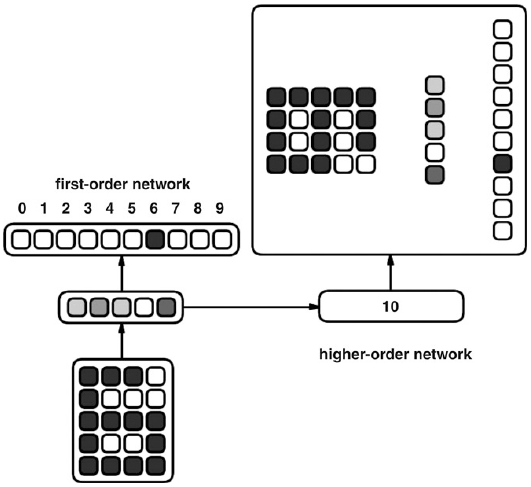
\includegraphics[width=220px]{data/expA1/schema.png}
      \end{center}
      
    \paragraph{Paramètres}
      \begin{center}
	\begin{tabular}{lr}
	  \begin{minipage}{230px}
	    \begin{itemize}
	      \item momentum : 0.9 sur les 2 réseaux
	      \item taux d'apprentissage : 0.1 sur les 2 réseaux
	      \item 10 chiffres différents présentés
	      \item apprentissage 10 (formes) x 1000 (époques)
	      \item utilisation de biais
	    \end{itemize}
	  \end{minipage}
	  &
	  \begin{minipage}{230px}
	    \begin{itemize}
	      \item poids initialisés sur [-0.25 ; 0.25]
	      \item taux d'apprentissage constant
	      \item entrées valent 0 ou 1
	      \item sigmoïde à température 1
	    \end{itemize}
	  \end{minipage}
	\end{tabular}
      \end{center}

  
  \newpage
  \subsection{Résultats}
    \paragraph{Principaux}
      Analyse des performances
      \begin{center}
	\begin{tabular}{lr}
	  \hspace*{-1cm}
	  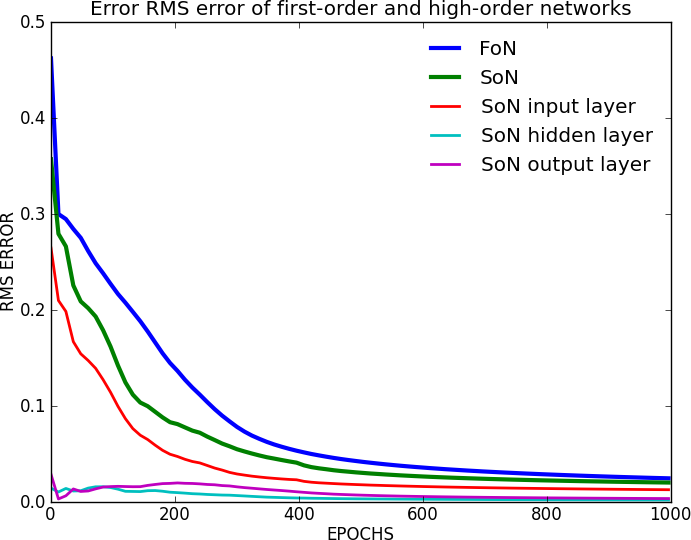
\includegraphics[width=250px]{data/expA1/rms.png}
	  &
	  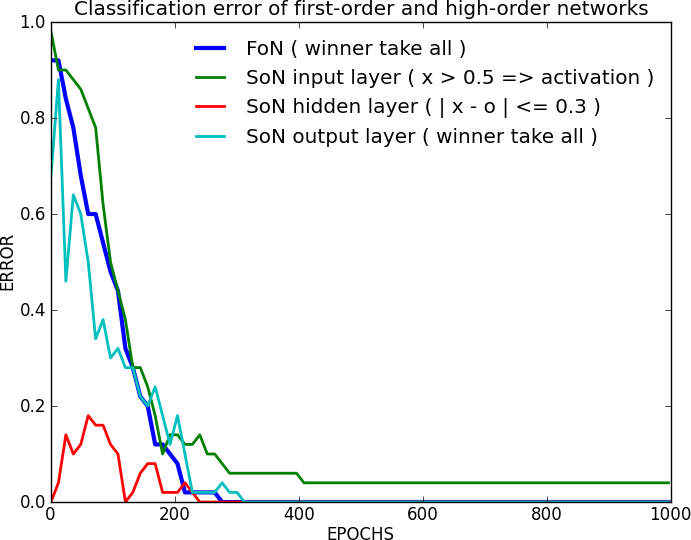
\includegraphics[width=250px]{data/expA1/err.png} 
	\end{tabular}
      \end{center}
      \subparagraph{Notes}
	\begin{itemize}
	  \item formule utilisée pour RMS (cf. Formules~\nameref{rms})
	  \item les courbes SoN layer représentent les erreurs (du second réseaux) sur les couches à reproduire 
	  \item la courbe RMS verte (SoN) est la somme des 3 courbes SoN layer
	  \item l'erreur de classification représente le taux de mauvaises réponses pour les 10 formes présentées sur une époque
	  \item pour SoN input layer et hidden layer, un winner-take-all n'est pas possible (ce n'est pas de la classification, 
	  mais une duplication), il y a donc un seuil d'erreur qui ne doit pas être dépassé par un seul neurone
	\end{itemize}
      \subparagraph{Conclusion}
	\begin{itemize}
	  \item le premier réseau réussit à apprendre sa tâche de classification
	  \item le second réseau réussit à apprendre sa tâche de duplication
	  \item la couche cachée et la couche de sortie ne posent aucun problèmes d'apprentissage
	  \item les performances du second réseau dépendent principalement de sa capacité à reproduire les entrées
	  \item le second réseau apprend plus rapidement que le premier
	\end{itemize}
    \paragraph{Secondaires}
      RMS indépendant par couche
      \begin{center}
	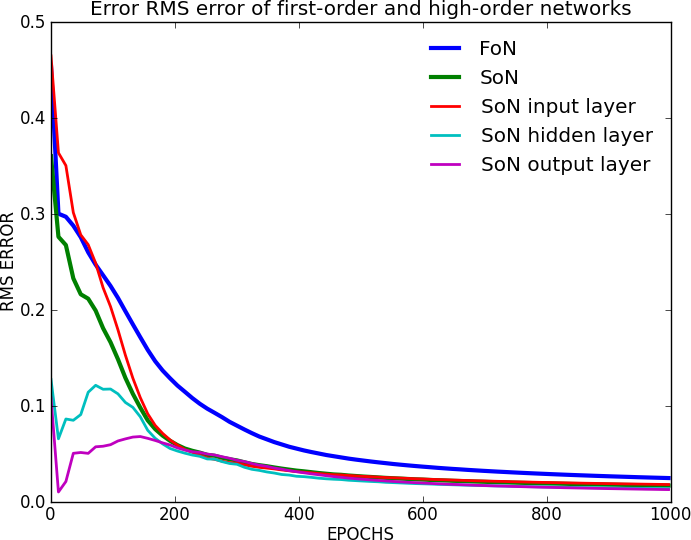
\includegraphics[width=250px]{data/expA1/rms_new.png}
      \end{center}
      \subparagraph{Notes}
	\begin{itemize}
	  \item formule utilisée pour RMS (cf. Formules~\nameref{rms})
	  \item les courbes SoN layer représentent les erreurs (du second réseaux) sur les couches à reproduire
	  \item les erreurs de SoN sont calculées en divisant par le nombre de neurone de la couche à reproduire (et non par le nombre total de neurones)
	\end{itemize}
      \subparagraph{Conclusion}
	\begin{itemize}
	  \item le SoN a plus de mal à apprendre la couche cachée que celle de sortie
	\end{itemize}
    \paragraph{Secondaires}
      Discrétisation de la couche cachée du premier réseau
      \begin{center}
	\begin{tabular}{lr}
	  \hspace*{-1cm}
	  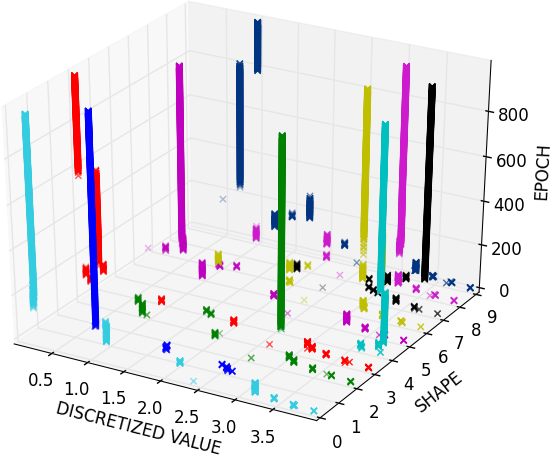
\includegraphics[width=250px]{data/expA1/discretize_cloud.png}
	  &
	  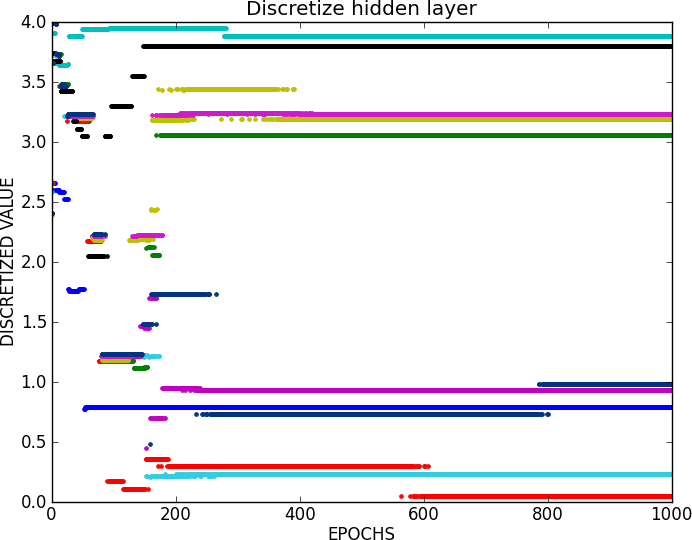
\includegraphics[width=250px]{data/expA1/discretize.png} 
	\end{tabular}
      \end{center} 
      \subparagraph{Notes}
	\begin{itemize}
	  \item une couleur équivaut à un chiffre présenté
	  \item une valeur discretisée correspond à un certain encodage de la couche cachée (cf Algorithmes~\nameref{discretize})
	\end{itemize}
      \subparagraph{Conclusion}
        On peut voir ici, qu'un simple perceptron permet de résoudre le problème ; puisqu'à la fin,
        aucunes des couleurs n'est superposées à une autre.
        
	Les neurones se stabilisent très rapidement (autour de la 50\up{ième} époque en moyenne), 
	le tout permettant au second réseau d'avoir des entrées très peu variables, favorisant
	son apprentissage.
    \paragraph{Secondaires}
      Représentations au travers des poids du premier réseau
      \begin{center}
	Couche cachée \\
	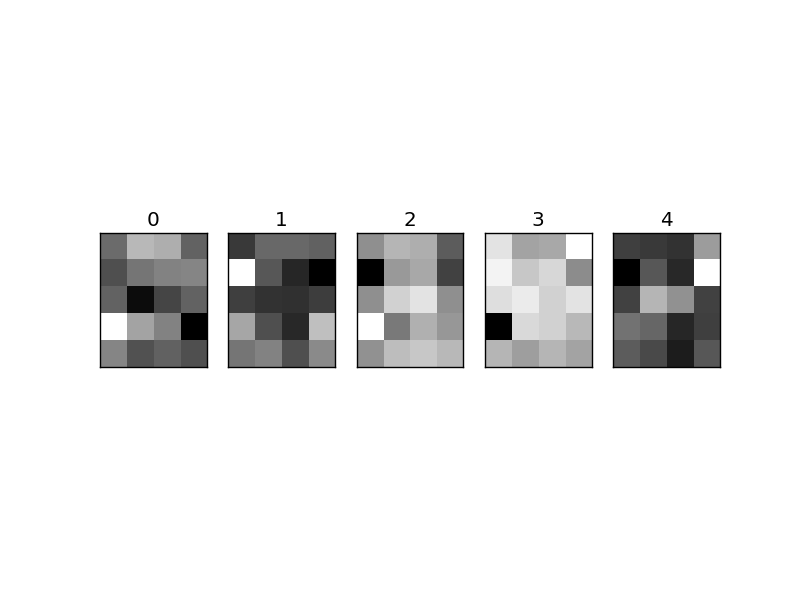
\includegraphics[width=250px]{data/expA1/representation_hidden.png}
      \end{center}
      \begin{center}
	Couche de sortie \\
	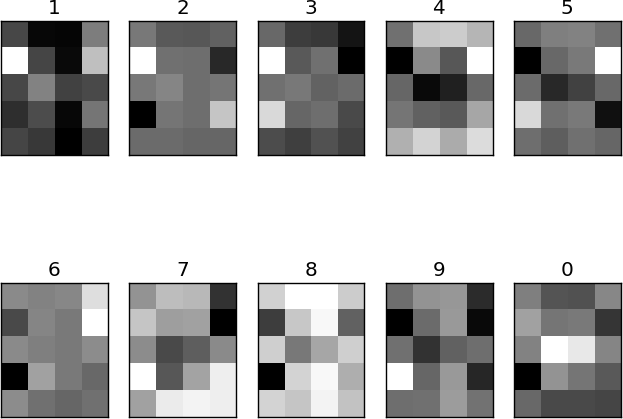
\includegraphics[width=250px]{data/expA1/representation.png}
      \end{center} 
      \subparagraph{Notes}
	\begin{itemize}
	  \item plus une case est noire, plus sa présence est importante pour le chiffre en question
	  \item plus une case est blanche, plus son absence est importante
	  \item c'est seulement lorsqu'elle est grise qu'elle n'est pas prise en compte
	\end{itemize}
      \subparagraph{Conclusion}
        Au vu du peu d'entrées différentes présentées au réseau (10), on peut voir qu'il fixe 3 à 4 points précis
        pour classifier un nombre.
    \paragraph{Secondaires}
      Prototypes à l'intérieur des neurones du second réseau qui essaient de redonner les entrées
      \begin{center}
	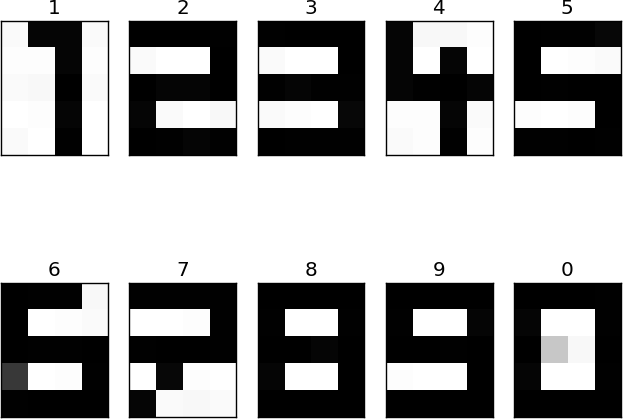
\includegraphics[width=250px]{data/expA1/prototype.png}
      \end{center} 
      \subparagraph{Notes}
	\begin{itemize}
	  \item Il sagit de la moyenne des réponses du second réseaux sur toutes les entrées
	\end{itemize}
      \subparagraph{Conclusion}
	Le peu d'entrées permet l'apprentissage par-coeur de chaque forme. À tel point qu'on ne peut pas vraiment
	parler de prototype.
	
  \subsection{Conclusion}
  Comme il l'est dit dans \cite{Cleeremans_2007}, cette architecture tente de résoudre les problèmes des réseaux connexionnistes
  classiques à avoir un semblant de conscience.
  
  À savoir :
  \begin{itemize}
   \item qu'ils ne savent pas qu'ils peuvent se trouver dans différents états, et qu'ils ne traitent pas leurs propres états : 
   d'où la présence de ce second réseau qui tente de traiter ses états et d'apprendre qu'il en a plusieurs
   \item des représentations restant bloquées dans la chaîne de causalité de la tâche à apprendre : d'où
   le fait que ce second réseau n'affecte pas l'apprentissage du premier (ie. pour ne pas retomber dans la chaîne de causalité)
   \\[0.2cm]
  \end{itemize}
  
  Au vu des résultats secondaires qui nous montre que la tâche est vraiment facile, dans l'\nameref{expA3},
  nous nous sommes intéressés à la même architecture mais sur des données réelles.
  
  Quant à l'\nameref{expB1}, nous avons expérimenté les représentations et le transfert de tâche.

  \newpage 
  \subsection{Formules}
    \paragraph{RMS} \label{rms}
  Pour une époque $e$ :
  \begin{center}
    \begin{large}
    $ rms_{e} = \sqrt{ \frac{1}{n} \sum \limits_{i=1}^{n} 
    ( o_{i,e} - d_{i} )^2 } $
    \end{large}
  $ with \left\lbrace \begin{array}{lll} n : number\ of\ neurons\ on\ the\ output\ 
  layer\\o_{i,e} : value\ obtained\ for\ the\ i^{th}\ neuron\ at\ the\ e^{th}\ epoch\\d_{i} : 
  value\ desired \ for\ the\ i^{th}\ neuron\end{array} \right.$
  \end{center}
    \paragraph{Discrétisation} \label{discretize}
      Pour la couche cachée $hiddenNeuron$ de $n$ neurones, un neurone
      pouvant être encodé par $number\_cutting$ valeurs différentes :
      \begin{center}
	$\sum \limits_{i=0}^{n} number\_cutting^{i} \times cutting(hiddenNeuron[i]) $
      \end{center}
      \subparagraph{Exemple}
	$400 \gets [0 ; 0,25 ]\ [0 ; 0,25 ]\  [0,25 ; 0,5 ]\  [0,5 ; 0,75 ]\  [0,25 ; 0,5 ]$ \\
	\hspace*{2.70cm}
	$400 \gets 0\times4^0 +   0\times4^1  +   1\times4^2   +  2\times4^3   +   1 \times4^4$
    \paragraph{Descente de gradient} \cite{Touzet_1992} \\
  Construction de l'erreur : 
    \begin{center}
      $y_{i} = f'(a_i) \times ( d_i - x_i ) \ si\ i\ neurone\ de\ sortie $ \\
      $y_{i} = f'(a_i) \times \sum \limits_{k} ( w_{ki} \times y_k )\ si\ i\ neurone\ cache $
    \end{center}
  Mise à jour des poids :
    \begin{center}
      $w_{ij}(t+1) = w_{ij}(t) + learning\_rate \times y_{i} \times x_j + momentum \times 
      (w_{ij}(t) - w_{ij}(t-1) )$
    \end{center}
  Variables : 
    \begin{center}
      $\left\lbrace \begin{array}{lll} 
	f : fonction\ sigmoide \\
	x_i : valeur\ du\ neurone\ i\\
	d_i : valeur\ desire pour\ le\ neurone\ i\\
	a_i : somme\ pondere\ des\ poids\ du\ neurone\ i
      \end{array} \right.$
    \end{center}
    
\bibliographystyle{../pre-rapport/apalike}
\bibliography{../pre-rapport/biblio}
